\chap{États: Pour ne pas toujours faire la même chose (avancé)}\label{ch.states}

Un programme VPL est composé d'une série de paires événement-action.
Tous les événements sont vérifiés périodiquement et les actions appropriées sont effectuées.
Ceci limite les programmes que nous pouvons créer ; pour aller plus loin nous avons besoin d'une façon de spécifier que certaines paires événement-action sont actives à un certain moment, alors que d'autres ne le sont pas.
Par exemple, dans le \cref{ch.line}, lorsque le robot sort de la ligne, nous aurions aimé qu'il tourne à gauche ou à droite afin de rechercher la ligne dans une direction qui dépend de quel côté il est sorti.

Les états sont disponibles dans le mode \emph{avancé} de VPL.
Cliquez sur \blksm{advanced} avant de travailler sur les projets de ce chapitre.

\sect{Tape, tape}

Dans les programmes que nous avons réalisé jusqu'ici, nous avons souvent \emph{démarré} Thymio en appuyant sur un de ces boutons et \emph{arrêté} Thymio en appuyant sur un autre.
Mais regardez votre ordinateur, normalement, il n'a qu'un seul bouton pour l'allumer ou l'éteindre.
%\blksm{power-button} 
Le bouton se \emph{rappelle} s'il est dans l'état \bu{allumé} ou l'état \bu{éteint}.
Le bouton inclut souvent une petite lumière qui indique son état courrant.

Écrivons un programme qui allume les lumières du robot si vous lui donnez une petite tape et qui les éteigne si vous lui donnez une seconde tape.

{\raggedleft \hfill Programme \bu{tap-allumé-éteint.aesl}}

Il est pratique de décrire ce comportemnet en utilisant un \textit{diagramme d'états} :

\begin{center}
\begin{picture}(240,45)
\thicklines
%\put(0,0){\framebox(240,40){}}
\put(20,20){\circle{40}}
\put(0,0){\makebox(40,40){\textsf{éteint}}}
\put(220,20){\circle{40}}
\put(200,0){\makebox(40,40){\textsf{allumé}}}
\put(40,30){\vector(1,0){160}}
\put(0,30){\makebox(240,10){\textsf{tape $\rightarrow$ allumer}}}
\put(200,10){\vector(-1,0){160}}
\put(0,10){\makebox(240,10){\textsf{tape $\rightarrow$ éteindre}}}
\end{picture}
\end{center}

Ce diagramme comprend deux états indiqués par des cercles, \bu{allumé} et \bu{éteint}.
Depuis l'état \bu{éteint}, le robot peut aller dans l'état \bu{allumé} et revenir, mais seulement en suivant les instructions sur les flèches.
Les instructions décrivent quand une transition d'un état à l'autre peut se produire et quand elle se produit :

\begin{itemize}

\item \textbf{Quand} Thymio est dans l'état \bu{éteint} \textbf{\textit{et}} que l'événement \emph{tape} se produit $\rightarrow$ \emph{allumer} le robot \textbf{\textit{et}} aller dans l'etat \bu{allumé}.

\item \textbf{Quand} Thymio est dans l'état \bu{allumé} \textbf{\textit{et}} que l'événement \emph{tape} se produit $\rightarrow$ \emph{éteindre} le robot \textbf{\textit{et}} aller dans l'etat \bu{éteint}.

\end{itemize}

L'accent mis sur le mot «\,\textbf{\textit{et}}\,» avant la flèche~$\rightarrow$ signifie que deux conditions doivent être remplies pour que la transition se fasse: (a) Le robot doit être dans un certain état et (b) l'événement doit se produire.
Lorsque les deux conditions sont remplies, alors la transition est prise ce qui fait à la fois changer l'état et exécute l'action écrite après la flèche~$\rightarrow$.

Il est important de réaliser que les deux parties de la condition sont indépendantes.
Dans le diagramme ci-dessus (répété ici) :

\begin{center}
\begin{picture}(240,45)
\thicklines
%\put(0,0){\framebox(240,40){}}
\put(20,20){\circle{40}}
\put(0,0){\makebox(40,40){\textsf{éteint}}}
\put(220,20){\circle{40}}
\put(200,0){\makebox(40,40){\textsf{allumé}}}
\put(40,30){\vector(1,0){160}}
\put(0,30){\makebox(240,10){\textsf{tape $\rightarrow$ allumer}}}
\put(200,10){\vector(-1,0){160}}
\put(0,10){\makebox(240,10){\textsf{tape $\rightarrow$ éteindre}}}
\end{picture}
\end{center}

l'événement \emph{tape} apparaît deux fois, mais l'action causée par cet événement \emph{dépend} de l'état dans lequel le robot se trouve.

De façon similaire, dans un même état, différents événements peuvent causer différentes actions et des transitions vers de nouveaux états différents.
Dans le diagramme suivant :

\begin{center}
\begin{picture}(300,80)
\thicklines
%\put(0,0){\framebox(240,80){}}
\put(25,42){\circle{40}}
\put(10,28){\makebox(30,30){\textsf{éteint}}}
\put(280,20){\circle{40}}
\put(265,6){\makebox(30,30){\textsf{allumé2}}}
\put(40,57){\vector(1,0){220}}
\put(280,65){\circle{40}}
\put(265,50){\makebox(30,30){\textsf{allumé1}}}
\put(40,27){\vector(1,0){220}}
\put(0,60){\makebox(295,10){\textsf{bouton gauche $\rightarrow$ s'allumer en vert}}}
\put(0,30){\makebox(295,10){\textsf{bouton droite $\rightarrow$ s'allumer en rouge}}}
\end{picture}
\end{center}

toucher le bouton gauche dans l'état \textbf{éteint} allumer le robot en vert et l'amène dans l'état \textbf{allumé1}, alors que toucher le bouton droite, \emph{dans le même état}, génère une action différente, allumer le robot en rouge, et amène le robot dans un état différent, \textbf{allumé2}.

\sect{Implémenter des diagrammes d'états avec des paires événement-action}

Nous montrons comment \emph{implémenter} le comportement décrit par le diagramme d'état avec des paires événement-action.
Implémenter signifie construire un programme qui fera ce que le diagramme d'états décrit.
La \cref{fig.turn-on-off} montre le programme.
Regardons maintenant les paires événement-action unes à unes.

\begin{figure}
	\subfigure[Une tape pour allumer ou éteindre]{
		\label{fig.turn-on-off1}
		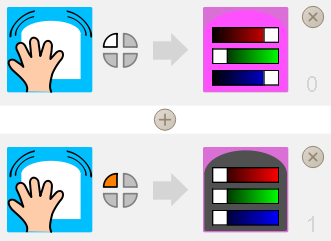
\includegraphics[width=.4\textwidth]{tap-on-off1}
	}
	\hfill
	\subfigure[Une tape pour changer d'état]{
		\label{fig.turn-on-off2}
		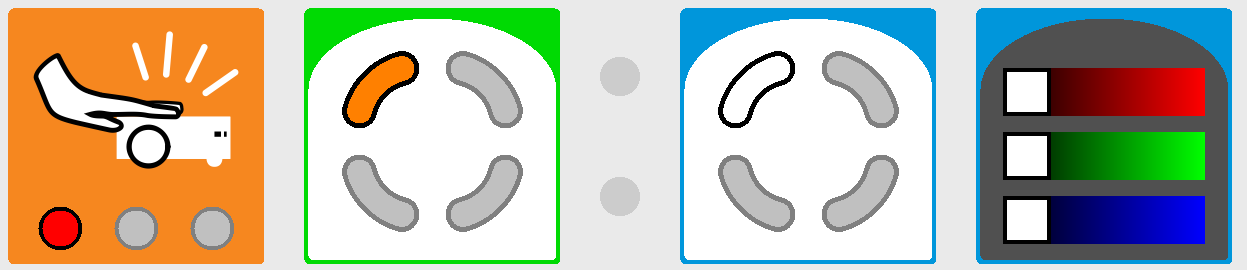
\includegraphics[width=.4\textwidth]{tap-on-off2}
	}
	\caption{Une tape qui a des résultats différents en fonction de l'état.}
	\label{fig.turn-on-off}
\end{figure}

Dans la première paire événement-action, l'événement est composé du bloc détection de choc avec une indication d'état \blksm{tap-turn-on-state-only}: \blkc{tap-turn-on}

Un état est indiqué par quatre quartiers d'un cercle, chacun pouvant être soit allumé (orange) ou éteint (blanc).
Dans ce programme, nous utiliserons le quartier en haut à gauche pour indiquer si la lumière du haut du robot est éteinte ou allumée.
Dans cette paire, ce quartier est coloré en blanc, ce qui veut dire que la lumière du robot est éteinte.
Ainsi, cette paire veut dire : si le robot est tapé et que le robot est éteint, allumer le robot.

La seconde paire événement-action veut dire : si le robot est tapé et qu'il est allumé, alors l'éteindre: \blkc{tap-turn-off}
% Ce quartier est coloré en orange, donc le robot est allumé 

Si vous regardez à nouveau le diagramme d'états, vous verrez que seulement la moitié du travail est fait.
En effet, en allumant et éteignant le robot, nous devons aussi changer son état d'\bu{éteint} à \bu{allumé} ou d'\bu{allumé} à \bu{éteint}.
Pour cela nous créons en plus deux paires événement-actions en utilisant le bloc d'action \emph{état} \blksm{action-states}, comme montré sur la \cref{fig.turn-on-off2}.

Le sens de la première paire est : \emph{quand} le robot est tapé \emph{et} que l'état est \emph{éteint}, alors changer l'état à \bu{allumé} : \blkc{tap-state-on}
De même, le sens de la seconde paire est : \emph{quand} le robot est tapé \emph{et} que l'état est \bu{allumé}, alors changer l'état à \bu{éteint} : \blkc{tap-state-off}

La \cref{fig.turn-on-off} montre le programme complet composé de quatre paires ; nous voyons que chaque événement cause à la fois une action sur la lumière et un changement de l'état du robot.
Tant l'action que le changement d'état dépendent de l'état dans lequel le robot se trouve, appellé \emph{état courrant}.

%\newpage

\sect{Dans combien d'états différents Thymio peut-il être?}

L'état est indiqué par un cercle divisé en quatre quartiers.
Quand utilisé avec un événement ou dans le bloc d'action état, chaque quartier peut être :
\begin{itemize}
	\item \textbf{Blanc}: le quartier est \emph{éteint} ;
	\item \textbf{Orange}: le quartier est \emph{allumé} ;
	\item \textbf{Gris}: le quartier n'est pas pris en compte.
\end{itemize}

Par exemple, dans \blksm{states}, les quartiers en haut à gauche et en bas à droite sont allumés, le quartier en haut à droite est éteint, et le quartier en bas à gauche n'est pas pris en compte.
Ceci veut dire que si \blksmpure{states} est associé à un bloc événement, l'événement se produira si l'état est défini soit par :
\begin{center}
\centering \makebox{\raisebox{-1.7em}{
\includegraphics[height=4em]{states1}}}\quad ou \quad \makebox{\raisebox{-1.7em}{
\includegraphics[height=4em]{states2}}}
\end{center}

Comme chacun des quatre quartiers peut être soit allumé soit éteint, il y a 2 $\times$ 2 $\times$ 2 $\times$ 2 = 16 états possibles :
\begin{quote}
\bu{(éteint, éteint, éteint, éteint)\\(éteint, éteint, éteint, allumé)\\(éteint, éteint, allumé, éteint)\\
\mbox{}\hspace{3em}\ldots\\
(allumé, allumé, allumé, éteint)\\
(allumé, allumé, allumé, allumé)}.
\end{quote}
La \cref{fig.all-states} énumère graphiquement tous ces états.
L'état courant du robot est toujours affiché sur le haut du robot par des arcs de cercles lumineux, par exemple, la \cref{fig.state-leds} montre le robot dans l'état \bu{(allumé, allumé, allumé, allumé)}.

\trickbox[Information]{Lorsqu'un programme démarre, l'état initial est toujours 
\bu{(éteint, éteint, éteint, éteint)}:\quad \blk{state-all-off}}

\trickbox{Si vous n'utiliser pas tous les 16 états possibles, mais par exemple que 2 ou 4, vous êtes libre de décider quel quartier vous utiliser pour représenter votre état.
Aussi, si par exemple vous avez deux choses différentes à encoder dans l'état, et que chacune d'elle a deux valeurs possibles, vous pouvez utiliser deux quartiers indépendemment.
C'est pourquoi la capacité d'\emph{ignorer} un quartier est très utile !
Essayez toujours de rester le plus simple possible.
}

\begin{figure}
	\subfigure[Tous les états possibles de Thymio]{
		\label{fig.all-states}
		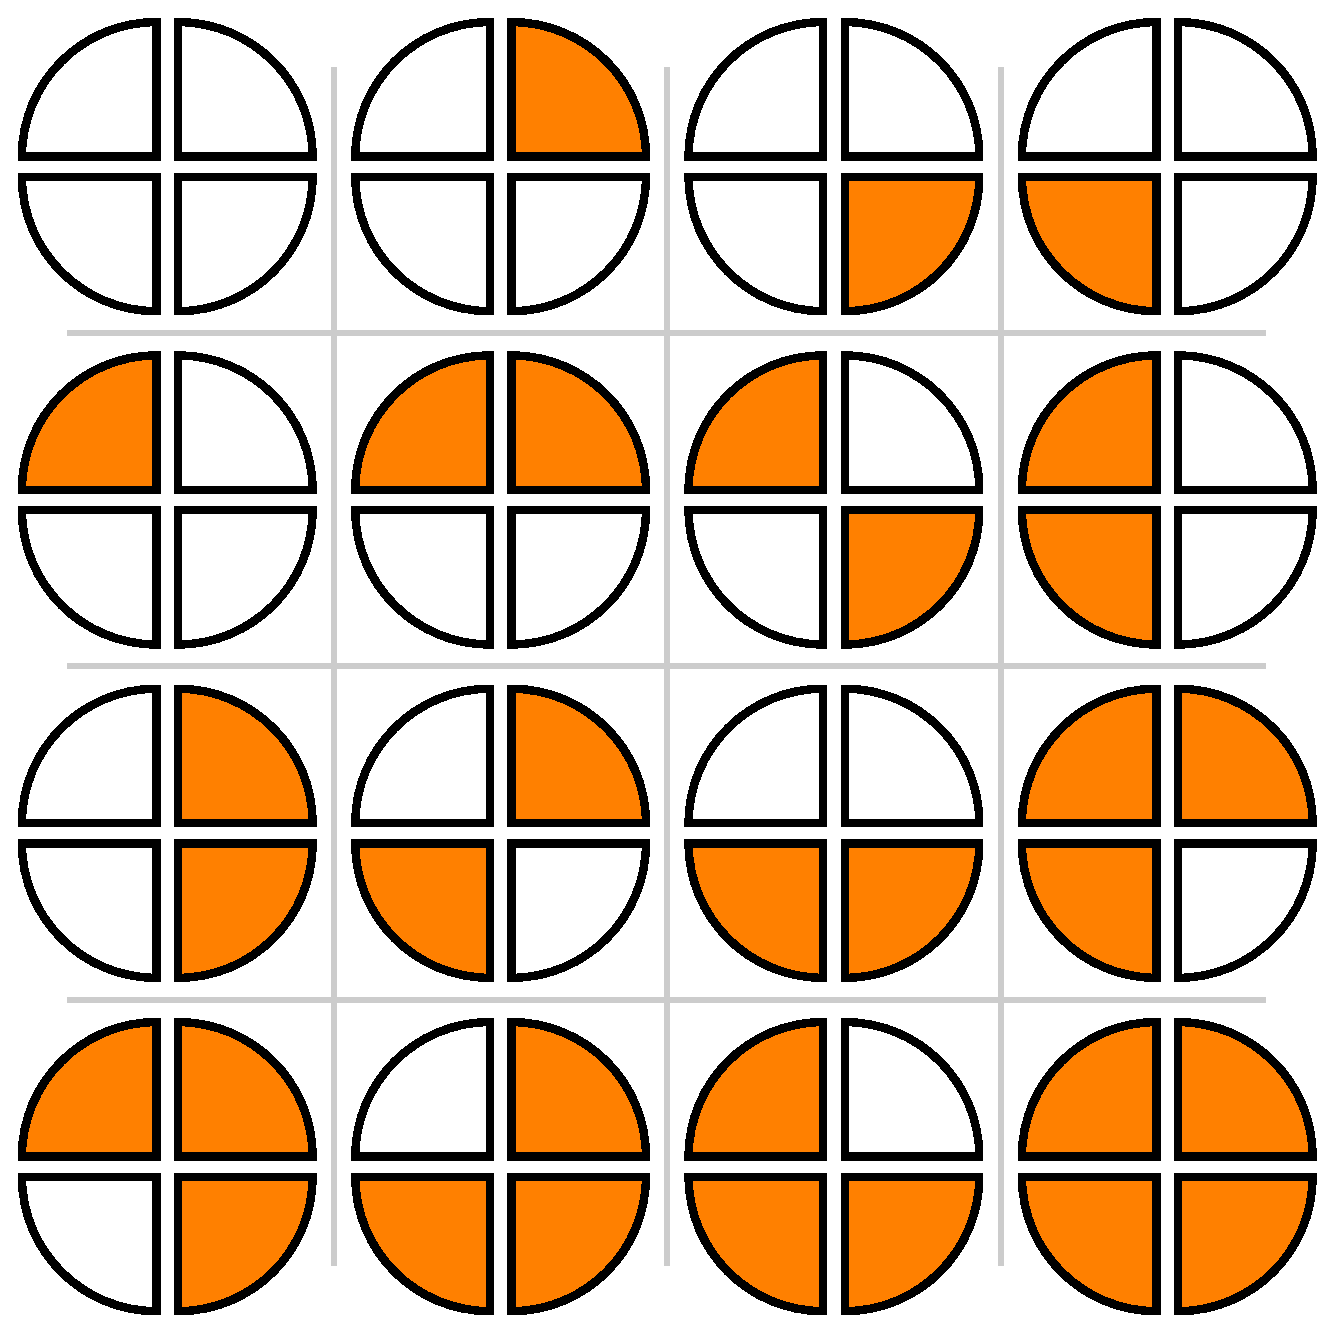
\includegraphics[width = 0.4\textwidth]{all-states}
	} 
	\hfill
	\subfigure[La cercle de LED indique l'état]{
		\label{fig.state-leds}
		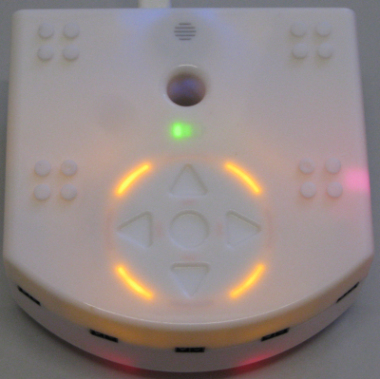
\includegraphics[width = 0.4\textwidth]{state-leds}
	}
	\caption{Les états de Thymio et leur représentation}
\end{figure}

\sect{Attraper la souris}

Écrivons un programme qui fasse tourner le robot de droite à gauche à la recherche d'une souris (ou d'un autre objet).
Si le robot détecte une souris avec son capteur avant-gauche, il continue la recherche jusqu'à ce que la souris soit détectée avec son capteur avant-droite.
Puis, il se positionne en face de la souris, comme sur la \cref{fig.cat-mouse}.

{\raggedleft \hfill Programme \bu{mouse.aesl}}

\begin{figure}
	\subfigure[Le chat a trouvé la souris]{\label{fig.cat-mouse}
	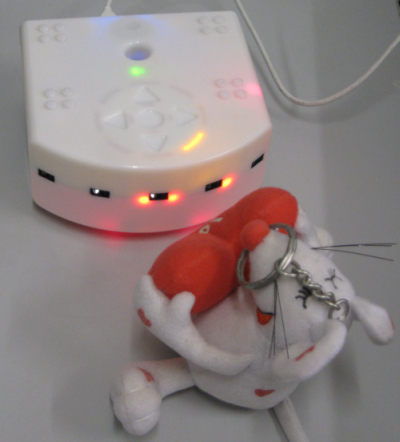
\includegraphics[width=0.4\textwidth]{cat-mouse}}
	\hfill
	\subfigure[Recherche avec le capteur avant-droite]{\label{fig.mouse2}
	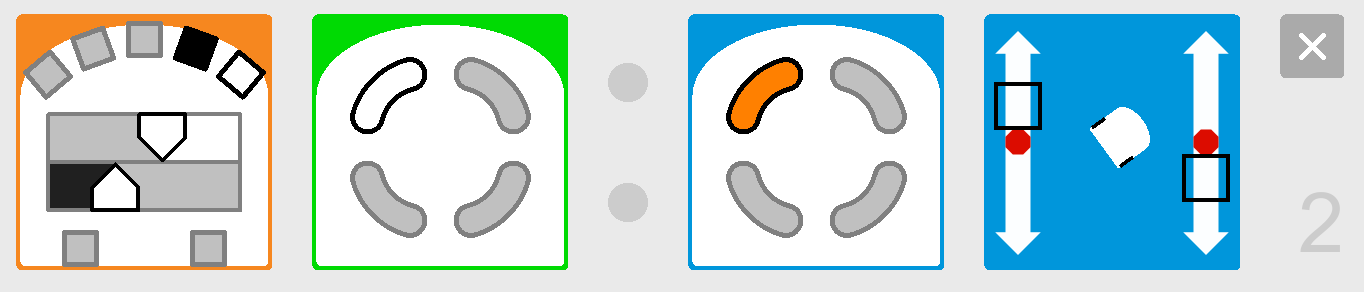
\includegraphics[width=0.4\textwidth]{mouse2}}
	\caption{Le robot chat cherche la souris}
\end{figure}

La paire événement-action suivante fait tourner le robot à gauche : \blkc{mouse1}
Ceci se produira lorsque le quartier gauche-haut est éteint ; initialement tous les quartiers de l'état sont éteint.

La première paire événement-action dans la \cref{fig.mouse2} attend que la souris soit détectée par le capteur avant-droite.
Notez que le petit carré à côté de ce capteur est blanc pour que l'événement se produise seulement si le capteur le plus à droite seul détecte la souris.
La seconde paire événement-action de la \cref{fig.mouse2} change l'état.

La dernière paire événement-action du programme arrête le robot lorsque la souris est directement en face du capteur avant-centre : \blkc{mouse3}
Pourquoi l'événement de cette paire doit-il dépendre de l'état ?
La raison est que le capteur central détectera aussi la souris durant le scan initial de droite à gauche.
Nous voulons que le robot fasse d'abord un scan complet avant de retourner à la position de la souris ; il est donc nécessaire que cette première détection soit ignorée.
Ceci est accomplit en arrêtant le scan seulement lorsque l'état est \bu{allumé} et ceci arrive que lorsqu'un scan complet a été effectué.

\vfill

\trickbox{
Il vous faudra expérimenter avec la distance de la souris au robot.
Si elle est trop proche du robot, les capteurs à côte du capteur central détecteront aussi la souris, alors que l'événement demande qu'ils ne la détecte \emph{pas}.
}

\vfill

\exercisebox{\thechapter.1}{
Écrivez un programme qui fasse danser le robot : il tourne à gauche sur place durant deux secondes, puis tourne à droite sur place durant trois secondes.
Ces mouvement se répètent indéfiniment.
}

\exercisebox{\thechapter.2 (Difficile)}{
Modifier le programme de suivi de ligne du \cref{ch.line} pour que le robot tourne à gauche quand il sort de la ligne par le côté droite, et qu'il tourne à droite quand il sort de la ligne par le côté gauche.
}